\documentclass{article}
\usepackage[utf8x]{inputenc}
\usepackage{ucs}
\usepackage{amsmath} 
\usepackage{amsfonts}
\usepackage{marvosym}
\usepackage{wasysym}
\usepackage{upgreek}
\usepackage[english,russian]{babel}
\usepackage{graphicx}
\usepackage{float}
\usepackage{textcomp}
\usepackage{hyperref}
\usepackage{geometry}
  \geometry{left=2cm}
  \geometry{right=1.5cm}
  \geometry{top=1cm}
  \geometry{bottom=2cm}
\usepackage{tikz}
\usepackage{ccaption}
\usepackage{multicol}

\hypersetup{
   colorlinks=true,
   citecolor=blue,
   linkcolor=black,
   urlcolor=blue
}

\usepackage{listings}
%\setlength{\columnsep}{1.5cm}
%\setlength{\columnseprule}{0.2pt}

\usepackage[absolute]{textpos}


\usepackage{colortbl,graphicx,tikz}
\definecolor{X}{rgb}{.5,.5,.5}

\renewcommand{\thesubsection}{\arabic{subsection}}

\begin{document}
\pagenumbering{gobble}
\lstset{
  language=C++,                % choose the language of the code
  basicstyle=\linespread{1.1}\ttfamily,
  columns=fixed,
  fontadjust=true,
  basewidth=0.5em,
  keywordstyle=\color{blue}\bfseries,
  commentstyle=\color{gray},
  stringstyle=\ttfamily\color{orange!50!black},
  showstringspaces=false,
  numbersep=5pt,
  numberstyle=\tiny\color{black},
  numberfirstline=true,
  stepnumber=1,                   % the step between two line-numbers.        
  numbersep=10pt,                  % how far the line-numbers are from the code
  backgroundcolor=\color{white},  % choose the background color. You must add \usepackage{color}
  showstringspaces=false,         % underline spaces within strings
  captionpos=b,                   % sets the caption-position to bottom
  breaklines=true,                % sets automatic line breaking
  breakatwhitespace=true,         % sets if automatic breaks should only happen at whitespace
  xleftmargin=.2in,
  extendedchars=\true,
  keepspaces = true,
}
\lstset{literate=%
   *{0}{{{\color{red!20!violet}0}}}1
    {1}{{{\color{red!20!violet}1}}}1
    {2}{{{\color{red!20!violet}2}}}1
    {3}{{{\color{red!20!violet}3}}}1
    {4}{{{\color{red!20!violet}4}}}1
    {5}{{{\color{red!20!violet}5}}}1
    {6}{{{\color{red!20!violet}6}}}1
    {7}{{{\color{red!20!violet}7}}}1
    {8}{{{\color{red!20!violet}8}}}1
    {9}{{{\color{red!20!violet}9}}}1
}
\newcommand\upquote[1]{\textquotesingle#1\textquotesingle}

\renewcommand{\thesubsection}{\arabic{subsection}}
\makeatletter
\def\@seccntformat#1{\@ifundefined{#1@cntformat}%
   {\csname the#1\endcsname\quad}%    default
   {\csname #1@cntformat\endcsname}}% enable individual control
\newcommand\section@cntformat{}     % section level 
\newcommand\subsection@cntformat{Задача \thesubsection.\space} % subsection level
\newcommand\subsubsection@cntformat{\thesubsubsection.\space} % subsubsection level
\makeatother


\makeatletter
\newcount\my@repeat@count
\newcommand{\myrepeat}[2]{%
  \begingroup
  \my@repeat@count=\z@
  \@whilenum\my@repeat@count<#1\do{#2\advance\my@repeat@count\@ne}%
  \endgroup
}
\makeatother

\title{Семинар \#7: Move-семантика и умные указатели. Домашнее задание.\vspace{-5ex}}\date{}\maketitle

\subsection{lvalue или rvalue}


Пусть есть следующий код:
\begin{lstlisting}
#include <cstdlib>

int funca()
{
    return 10;
}

int& funcb(int& x)
{
    x = x + 1;
    return x;
}

int&& funcc(int& x)
{
    x = x + 1;
    return static_cast<int&&>(x);
}

int main()
{
    int a = 100;
    int& l = a;
    int&& r = 200;
    
    // Мы находимся тут
}
\end{lstlisting}

Какие из следующих выражений являются lvalue, а какие - rvalue:

\begin{multicols}{3}
\begin{enumerate}
\item \texttt{100}
\item \texttt{a}
\item \texttt{a + 1}
\item \texttt{l}
\item \texttt{r}
\item \texttt{l + r}
\item \texttt{std::abs(a)}
\item \texttt{funca()}
\item \texttt{funcb(a)}
\item \texttt{funcb(l)}
\item \texttt{funcb(r)}
\item \texttt{funcc(a)}
\item \texttt{funcc(l)}
\item \texttt{funcc(r)}
\item \texttt{static\_cast<int>(a)}
\item \texttt{static\_cast<int\&>(a)}
\item \texttt{static\_cast<int\&\&>(a)}
\item \texttt{static\_cast<int\&\&>(r)}
\item \texttt{rand() > 5 ? a : 10}
\item \texttt{rand() > 5 ? a : r}
\item \texttt{+a}
\end{enumerate}
\end{multicols}

Решение этой задачи -- текстовый файл с ответами.

\newpage
\subsection{Стек строк}
Напишите класс \texttt{StringStack}, объекты которого будут хранить некоторое количество строк типа \texttt{std::string}.
Нужно написать следующие методы класса \texttt{StringStack}:

\begin{itemize}
\item \texttt{push}: В этот метод передаётся одна строка и эта строка добавляется в стек. Причём, если строка передаёся по lvalue, то она должна скопироваться, а если по rvalue, то переместиться.
\item \texttt{print}: Этот метод должен печатать на экран все элементы стека в скобках, через запятую.
\item \texttt{pop}: Этот метод должен удалять из стека последний элемент и возвращать его. В этом случае не должно происходить копирования строк, а только перемещения.
\end{itemize}

Напишите этот класс БЕЗ использования rvalue ссылок и универсальных ссылок.
Используйте стандартные классы \texttt{std::string} и \texttt{std::vector} внутри класса это сильно упростит задачу.

\begin{lstlisting}
...
StringStack ss;
std::string a {"Cat"};

ss.push(a);                    // должен скопировать строку a внутрь объекта ss
ss.push(std::string{"Mouse"}); // должен переместить временную строку внутрь объекта ss
ss.print();                    // печатает  (Cat, Mouse)
cout << a << endl;             // печатает  Cat

ss.push(std::move(a));         // должен переместить строку a внутрь объекта ss
ss.print();                    // печатает  (Cat, Mouse, Cat)
cout << a << endl;             // скорей всего напечатает  пустую строку 
                               // ( зависит от длины строки и компилятора )

cout << a.pop() << endl;       // печатает  Cat
ss.print();                    // печатает  (Cat, Mouse)
cout << a.pop() << endl;       // печатает  Mouse
cout << a.pop() << endl;       // печатает  Cat
ss.print();                    // печатает  ()
...
\end{lstlisting}


\newpage
\subsection{Разделитель по категориям}
Напишите класс \texttt{CategorySeparator}, который будет хранить в себе некоторое количество строк.
Причём он должен запоминать, какие строки добавлялись как lvalue-выражения, а какие строки, как rvalue-выражения. Нужно написать следующие методы класса \texttt{CategorySeparator}:

\begin{itemize}
\item \texttt{push}: В этот метод передаётся одна строка (lvalue или rvalue) и эта строка добавляется в разделитель.
\item \texttt{printLvalues}: Этот метод должен печатать на экран строки, которые были добавлены в разделитель как lvalue-выражения.
\item \texttt{printRvalues}: Этот метод должен печатать на экран строки, которые были добавлены в разделитель как rvalue-выражения.
\end{itemize}

Используйте стандартные классы \texttt{std::string} и \texttt{std::vector} внутри класса это сильно упростит задачу.
\begin{lstlisting}
...
CategorySeparator cs;
std::string a {"Cat"};
std::string b {"Dog"};

cs.push(a);                     // должен скопировать строку a внутрь объекта cs
cs.push(std::string{"Mouse"});  // должен переместить временную строку внутрь объекта cs
cs.push(a + b);                 // должен переместить временну строку a + b внутрь объекта cs
cs.push(b);                     // должен скопировать строку b внутрь объекта cs
cs.push(std::move(b)); 	        // должен переместить строку b внутрь объекта cs

std::cout << a << std::endl;    // печатает "Cat"
std::cout << b << std::endl;    // скорей всего напечатает  пустую строку 
                                // ( зависит от длины строки и компилятора )

cs.printLvalues();              // печатает  "(Cat, Dog)"
cs.printRvalues();              // печатает  "(Mouse, CatDog, Dog)"
...
\end{lstlisting}



\newpage
\subsection{Односвязный список, используя \texttt{std::unique\_ptr}}
Создайте шаблонный класс \texttt{ForwardList<T>}, при этом, поле в узле списка, которое будет указывать на следующий узел должно иметь тип \texttt{std::unique\_ptr}. Поля такого класса должны выглядеть так:

\begin{lstlisting}
template <typename T>
class ForwardList
{
    struct Node
    {
        T value;
        std::unique_ptr<Node> next;
    };
    
    std::unique_ptr<Node> mpHead;
    Node* mpTail;
	...
};
\end{lstlisting}

Схематическое строение объекта такого класса:

\begin{center}
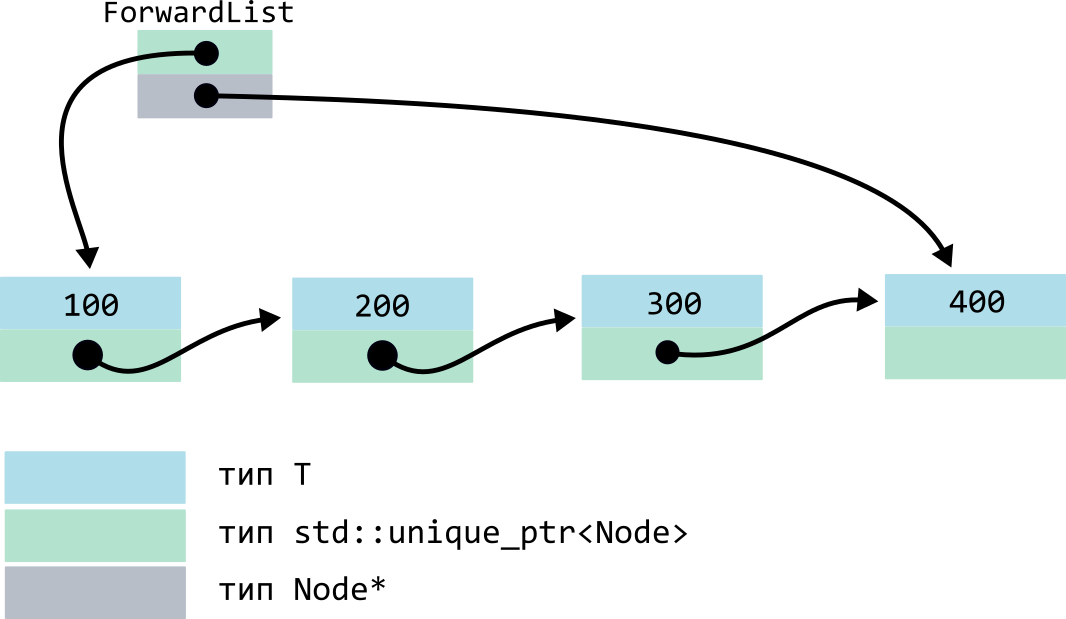
\includegraphics[scale=1]{../images/forward_list_unique.png}
\end{center}

Вам нужно написать следующие методы данного класса:

\begin{itemize}
\item Конструктор по умолчанию.
\item \texttt{void print()}
\item \texttt{void push\_front(T elem)}
\item \texttt{void push\_back(T elem)}
\item \texttt{std::unique\_ptr<T> pop\_front()}
\item \texttt{std::unique\_ptr<T> pop\_back()}
\item \texttt{void clear()}
\item \texttt{template <typename F> void foreach(F f)} -- применяет функцию \texttt{f} к каждому элементу связного списка. Функция f должна принимать объект типа \texttt{T} по обычной ссылке.


\item \texttt{void swap(ForwardList\& fl)} - меняет местами содержимое данного связного списка и списка \texttt{fl}.
\item \texttt{ForwardList copy()} - возвращает полную копию данного связного списка.
\end{itemize}


\end{document}
